\section{Transient Absorption}
\label{sec:TRAS}


\begin{table}[ht]
    \centering
    \begin{tabular}{clc}
        \toprule
        Sample No. &    Treatment &    $\tau$ / \si{\nano\second} \\
        \midrule
        1 &     ZnTPP in BN 0.8mM &  $953 \pm 3$ \\
        2 &     ZnTPP in BN 0.6mM &  $972 \pm 4$ \\
        3 &     ZnTPP in BN 0.4mM & $1000 \pm 4$ \\
        4 &     ZnTPP in BN 0.2mM & $1008 \pm 8$ \\
        5 & ZnTPP:C70 in BN 1:0.1 &  $834 \pm 3$ \\
        6 & ZnTPP:C70 in BN 1:0.2 &  $753 \pm 3$ \\
        7 & ZnTPP:C70 in BN 1:0.3 &  $697 \pm 3$ \\
        8 &    ZnTPP in Tol 0.8mM &  $533 \pm 1$ \\
        12 &     ZnOEP in BN 0.8mM &  $373 \pm 1$\\
        \bottomrule
    \end{tabular}
\end{table}



\subsection*{Variation in Concentration}
For ZnTPP, different concentrations in BN were measured. From the theory, we expect an exponential decay of the concentration of the triplet 
\begin{equation}
    C_T(t) = C_T(0) \exp[-k_0t],
\end{equation}
with the initital concentration $C_T(0)$ and the decay rate $k_0$.
As the transient absorption $\Delta A(\tau)$ is proportional to $C_T$, we can fit an exponential decay to our data. Hereby, an offset was added to the decay function to correct any offset caused by e.g.~measuring methods. Data and fits are shown in fig.~\ref{fig:TRAS-Conc}.

\begin{figure}[h]
    \centering
    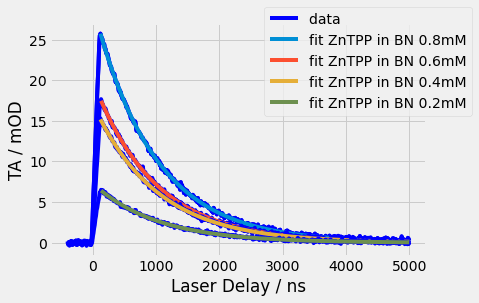
\includegraphics[width = \textwidth]{Bilder/Auswertung/TRAS/ZnTPPdiffConc.png}
    \caption{Data of the transient absorption of solutions of different concentrations of ZnTPP in BN.}
    \label{fig:TRAS-Conc}
\end{figure}

It is clear, that higher maxima correspond to higher concentrations of ZnTPP. This aligns our expectations as a higher concentration leads to a bigger ammount of absorption. The lifetime $\tau_0$ can be calculated from 
\begin{equation}
    \tau_0 = \frac{1}{k_0}.
\end{equation}

The calculated lifetimes can be found in tab.~\ref{tab:lifetimesConc}.

\begin{table}[ht]
    \centering
    \begin{tabular}{clc}
        \toprule
        Sample No. &    Treatment &    $\tau$ / \si{\nano\second} \\
        \midrule
        1 &     ZnTPP in BN 0.8mM &  $953 \pm 3$ \\
        2 &     ZnTPP in BN 0.6mM &  $972 \pm 4$ \\
        3 &     ZnTPP in BN 0.4mM & $1000 \pm 4$ \\
        4 &     ZnTPP in BN 0.2mM & $1008 \pm 8$ \\
        \bottomrule
    \end{tabular}
    \caption{Calculated lifetimes of ZnTPP solutions in BN with different concentrations.}
    \label{tab:lifetimesConc}
\end{table}